\chapter{Metodología}

\section{Descripción de los datos}

\noindent Las series temporales de campo magnético del viento solar provienen de mediciones in situ realizadas por las sondas espaciales PSP y SolO durante su primer alineamiento radial a una distancia de $ \sim 0.1 UA$ y $ \sim 1 UA$, respectivamente. Los datos de la sonda PSP fueron registrados el 27 de septiembre de 2020 desde las 03:05 UT hasta las 05:15 UT (130 minutos), y los datos de la sonda SolO fueron tomados el 01 de octubre de 2020 a las 21:20 UT hasta el 02 de octubre de 2020 a las 01:20 UT (240 minutos). La frecuencia de muestreo de los datos estudiados es de 8 $Hz$.  

\begin{figure}[H]
    \centering
    \includegraphics[scale=0.45]{data_PSP.png}
    \caption{Datos del campo magnético en la sonda PSP durante el intervalo de tiempo 03:05 - 05:15 UT el 27 de septiembre de 2020. De arriba hacia abajo: $B_{R}$ y $|B|$, $B_{T}$ y $B_{N}$.}
    \label{fig1}
\end{figure}

En las figuras \ref{fig1} y \ref{fig2} se muestra la intensidad de campo magnético ($|B|$) y sus componentes en el sistema de coordenadas RTN, para las series temporales de ambas sondas espaciales. En el sistema de coordenadas RTN, la componente R apunta radialmente desde el centro del Sol hasta la nave espacial; la componente tangencial T es el producto cruz de la velocidad angular del Sol con R; y la componente normal N completa la triada ortogonal y tiene la misma dirección que la velocidad angular del Sol \cite{bruno_turbulence_2016}.

\begin{figure}[H]
    \centering
    \includegraphics[scale=0.45]{data_SolO.png}
    \caption{Datos del campo magnético en la sonda SolO desde el 01 de octubre de 2020 a las 21:20 UT hasta el 02 de octubre de 2020 a las 01:20 UT. De arriba hacia abajo: $B_{R}$ y $|B|$, $B_{T}$ y $B_{N}$.}
    \label{fig2}
\end{figure}

\section{Empirical Mode Decomposition}\label{EMD}

\noindent Muchos de los fenómenos físicos en la naturaleza se caracterizan por tener una dinámica no lineal \cite{strogatz_nonlinear_2015} y, en muchas ocasiones, no estacionaria. Incluso el ejemplo más sencillo que se le puede ocurrir a un físico, como es el movimiento de un péndulo simple en ausencia de fuerzas externas y rozamiento es, en general, no lineal. Además, aún en el caso de pequeñas oscilaciones, cuando se considera un movimiento amortiguado, se pierde la estacionariedad, pues la amplitud de oscilación deja de ser constante y su valor medio cambia con el tiempo \cite{Priestley, chatfield_analysis_2019}.        

Los datos de series temporales pueden mostrar diversos patrones que son más fáciles de entender cuando se descomponen en varios componentes. Es como observar un reloj y tener una idea de cómo funciona, pero solamente entenderlo (o mejorar la comprensión) cuando se lo desarma y observa la posición de sus partes y cómo estas interactúan entre sí. De igual manera, descomponer una señal puede hacer más fácil su análisis cuando se hace uso de las técnicas adecuadas. Por ejemplo, la transformada de Fourier permite identificar las componentes de frecuencia de una señal y, operando sobre estas, filtrar las frecuencias \cite{rao_fast_2010} que no sean de interés.   

Los métodos estándar basados en la transformada de Fourier y la transformada Wavelet son muy utilizados para analizar series temporales pues están basados en una teoría matemática robusta \cite{huang_empirical_1998, Percival}, lo que facilita la interpretación de los resultados. Sin embargo, las teorías analíticas que soportan estos métodos requieren de propiedades de ortogonalidad y/o completitud, lo que fija a priori el número de componentes en las que se descompone una señal. Más aún, estas componentes pueden tener otras restricciones adicionales como ser funciones sinusoidales, el cual es el caso en la transformada de Fourier con los modos de oscilación armónicos. 

En una serie temporal cualquiera puede que su descomposición no sea idónea en componentes sinusoidales. Tampoco puede que exista un número fijo para el cual se obtenga una clara distinción entre ellas. Este es el caso de las series temporales que provienen de sistemas físicos no lineales, no estacionarios y que pueden tener diferentes escalas características. Por esta razón, el análisis y la descripción de estos sistemas requiere el uso de diferentes métodos basados en técnicas adaptativas que permitan describir sus características inherentes a partir de una descomposición basada en los propios datos.

El método Empirical Mode Decomposition (EMD) es un método adaptativo que se basa en la escala de tiempo característica local de los datos, permitiendo descomponer señales de procesos no lineales y no estacionarios \cite{huang_empirical_1998}. Es decir, este método analiza las características de los datos de punto a punto para realizar la descomposición sin importar si los procesos son no lineales o no estacionarios. Además, como el método está basado en los datos, la base de la descomposición se define a posteriori y no se imponen restricciones sobre estas componentes (amplitud constante y frecuencia fija en el caso de la expansión de Fourier). El EMD permite descomponer una señal en un número finito de componentes oscilatorias denominadas funciones de modo intrínseco (Intrinsic Mode Functions, IMFs), las cuales poseen amplitud y frecuencia moduladas. 

La descomposición de una serie temporal en sus IMFs se realiza mediante un proceso iterativo denominado \textit{sifting} (tamizado). El razonamiento detrás de este proceso consiste en extraer los componentes de una señal comenzando con aquellas de mayor frecuencia y con cada iteración separar los diferentes modos de una señal según sus características para de esta manera terminar con la IMF con menor frecuencia. Esto es similar a tener un arreglo de tamices diferentes. Al finalizar este proceso la serie temporal original $x(t)$ puede escribirse como la suma de $M$ modos oscilantes $c_{j}(t)$ (IMFs) y un residuo monótono $r(t)$, que representa la tendencia a largo plazo de la señal original, lo cual es usual en el análisis de series temporales \cite{chatfield_analysis_2019}. 

\begin{equation}
    x(t) = \sum_{j=1}^{M} c_{j}(t) + r(t)
    \label{emd}
\end{equation}

\newpage

Las IMFs que se obtienen tras la descomposición poseen dos propiedades importantes.

\begin{enumerate}[label=(\arabic*)]
    \hypertarget{imfs_cond1}{\item} El número de extremos y cruces por cero es igual o difieren como máximo en uno. 
    \hypertarget{imfs_cond2}{\item} El valor medio es cero. 
\end{enumerate}

La primera condición garantiza que no existan oscilaciones complicadas en las componentes de la descomposición y que exista un cruce por cero al menos una vez antes de que pasar de un extremo a otro, lo que dota a las IMFs de simetría y hace que el método sea adaptativo. Por otro lado, la segunda condición permite obtener frecuencias instantáneas que no sean afectadas por fluctuaciones asimétricas. Esto también implica que las IMFs son estacionarias (lo cual permite ampliar el análisis de las series temporales \cite{huang_amplitude-frequency_2008}). De esta manera, cada IMF tiene una amplitud modulada y frecuencias instantáneas físicamente significativas que pueden ser de banda estrecha \cite{huang_empirical_1998}.  

El proceso \textit{sifting} es la base del método EMD y los pasos que se utilizaron en este trabajo pueden resumirse en el siguiente algoritmo:    

\begin{spacing}{1}
    \begin{enumerate}[label=\arabic*.]
        \item Establecer la condición inicial para el residuo $r(t) = x(t)$.
        \item Identificar los máximos y mínimos locales de $x(t)$. 
        \item Usar la interpolación cubic splines para calcular las envolventes, superior $e_{max}(t)$ e inferior $e_{min}(t)$, definidas por los máximos y mínimos locales, respectivamente.  
        \item Calcular la envolvente media $e_{m}(t) = \frac{1}{2}(e_{min}(t) + e_{max}(t))$.
        \item Evaluar $h_{i}(t) = x(t) - e_{m}(t)$, denominada proto-IMF, y verificar si cumple con las condiciones \hyperlink{imfs_cond1}{(1)} y \hyperlink{imfs_cond2}{(2)} para ser una IMF.
        \item Si $h_{i}(t)$ es una IMF entonces $c_{j}(t) = h_{i}(t)$ se guarda y se actualiza el residuo $r(t) = r(t) - c_{j}(t)$, de lo contrario se repiten los pasos del 2 al 5 sobre $x(t)' = h_{i}(t)$ hasta obtener una IMF.    
    \end{enumerate}
\end{spacing}

Las iteraciones en el proceso \textit{sifting} son limitadas puesto que de lo contrario las IMFs pierden sentido físico, dado que esto puede eliminar las características locales de las series. Desde la presentación del método EMD se han propuesto y utilizado diferentes criterios de detenimiento \cite{rilling_empirical_nodate, flandrin_empirical_2004, de_michelis_multi-scale_2012}. En este trabajo solamente se utiliza el criterio que fue propuesto originalmente. Este criterio establece que el proceso \textit{sifting} se detiene cuando $SD<SD^{*}$, donde

\begin{equation}
    SD = \sum_{t=1}^{T} \dfrac{|h_{i}(t) - h_{i-1}(t)|^2}{h_{i-1}^{2}(t)},  \; i>1
    \label{SD_criterion}
\end{equation}

$T$ es la duración de la serie temporal (``longitud” de los datos) y $SD^{*}$ es un valor límite que puede tomar valores entre $0.2$ y $0.3$ \cite{huang_empirical_1998}.

Cada vez que el proceso \textit{sifting} encuentra una IMF se verifica el número de extremos del residuo $r(t)$, definido en el paso 6 del algoritmo, para determinar si la descomposición finaliza. El residuo representa la tendencia media de la serie temporal $x(t)$ y puede ser una función constante o monótona. Por tanto, el método EMD termina cuando el residuo tiene como máximo un extremo o se cumple algún otro criterio de detenimiento.

La descomposición que realiza el método EMD genera $\sim \log_{2}(N)$ IMFs, donde $N$ es el número de puntos de la serie temporal. Esto es porque en el caso de ruido estocástico de banda ancha, el EMD actúa como un banco de filtros diádicos \cite{flandrin_empirical_2004} (arreglo de filtros pasa banda que reduce en un factor de 2 la salida de cada filtro \cite{ filter_banks}). A través de esta aproximación, en este trabajo se impuso un máximo al número esperado de IMFs y con la condición de que el residuo tenga a lo mucho un extremo, finalizar la descomposición de los datos.   

La implementación del método EMD en Fortran se hizo en doble precisión y se adjunta en el anexo \ref{EMD_code}. Sin embargo, en la verificación de las condiciones del residuo se redujo la precisión a la mitad debido a que de lo contrario el algoritmo seguía iterando y generando más componentes que ya no eran IMFs.

En este trabajo se tomó $SD^{*} = 0.3$ como el valor límite para el criterio de detenimiento del proceso \textit{sifting}. En la implementación realizada en Fortran, junto a esta condición, también se fijó un número máximo de iteraciones, pues de lo contrario este número se hacía muy grande. Como se mencionó, esto puede hacer que las IMFs pierdan relevancia física. Además, como los resultados no variaron mucho para un número de iteraciones similar al número esperado de IMFs ($\sim 16$ para PSP y $\sim 17$ para SolO), se tomaron $20$ iteraciones como el número máximo de iteraciones del proceso \textit{sifting} para descomponer los datos de las series temporales del campo magnético.

\subsection{Cubic Splines}

\noindent Evaluar las envolventes de los extremos locales es un paso importante para el cálculo de las IMFs. Se han estudiado algunas formas de realizar la interpolación sobre los extremos para estimar las envolventes, pero la interpolación mediante cubic splines es la más utilizada \cite{huang_empirical_1998, rilling_empirical_nodate}. A continuación, se explica brevemente la idea detrás de este método de interpolación.   

La interpolación cubic splines permite ajustar localmente un conjunto de puntos a una función a trozos de tal manera que cada parte se conecte suavemente. Esta interpolación se realiza mediante polinomios de tercer grado haciendo coincidir la función y sus derivadas en los puntos de datos que conectan los trozos de la función \cite{pang_introduction_2006}. Así, para un conjunto discreto de $n+1$ puntos $(x_{i}, y_{i})$, descritos por una función $f$ en el intervalo $[a, b]$ tal que $y_{i} = f(x_{i})$ y $a = x_{0}<x_{1}< \ldots < x_{n} = b$, una función $S$ es un cubic splines si satisface las siguientes condiciones \cite{young_introduction_nodate}:

\begin{enumerate}[label=\arabic*.]
    \item En el intervalo $[x_{i}, x_{i+1}]$, $S(x)$ es un polinomio de tercer grado denotado por $S_{i}(x), \; i = 0, 1, \ldots, n-1$.  
    \item $S_{i}(x_{i}) = y_{i}$ y $S_{i}(x_{i+1}) = y_{i+1}, \; i = 0, 1, \ldots , n-1$.
    \item $S'_{i}(x_{i+1}) = S'_{i+1}(x_{i+1}), \;  i = 0, 1, \ldots , n-2$.
    \item $S''_{i}(x_{i+1}) = S''_{i+1}(x_{i+1}), \;  i = 0, 1, \ldots , n-2$. 
\end{enumerate}

En cada intervalo la función de cubic splines toma la forma $S_{i}(x) = a_{i} + b_{i}x + c_{i}x^2 + d_{i}x^3, \; i=0, 1, \ldots, n-1$, y los coeficientes se determinan mediante las condiciones de frontera. En total se tienen $4n$ incógnitas, pero $4n-2$ ecuaciones, por lo que para cerrar el sistema se pueden utilizar algunas condiciones adicionales. En este trabajo se utilizó las denominadas condiciones de frontera naturales, las cuales son $S''_{0}(x_{0}) = S''_{n-1}(x_{n}) = 0$ \cite{pang_introduction_2006, young_introduction_nodate}.    
  
En la figura \ref{fig:cubic_splines} se muestra el uso de la interpolación cubic splines para evaluar las envolturas de los máximos y mínimos locales de una función de prueba $f$. El cálculo de los extremos no considera los puntos al inicio y al final de la función, por lo que las envolventes divergen en estos puntos. Por este motivo, para que el proceso \textit{sifting} se realice de manera adecuada, se deben imponer condiciones de frontera adicionales sobre los máximos y mínimos de los datos.         

\begin{figure}[H]
    \centering
    \includegraphics[scale=0.6]{cubic_splines.png}
    \caption{Envoltura de los máximos $e_{max}(x)$ y mínimos $e_{min}(x)$ locales, y su valor medio $e_{m}(x)$, de la función de prueba $f$ mediante la interpolación cubic splines.}
    \label{fig:cubic_splines}
\end{figure}

\subsection{Condiciones de frontera en el cálculo de las envolventes}

\noindent La evaluación adecuada de las envolventes al inicio y al final de los datos se resaltó desde que se presentó el método. Las condiciones de frontera seleccionadas permiten mitigar la propagación de ondas complejas desde los puntos en los extremos hacia el interior de las IMFs. Asimismo, esto es importante para que la interpolación permita obtener mejores resultados, puesto que los métodos de interpolación suelen realizar suposiciones para tener un sistema de ecuaciones cerrado. Por ejemplo, en el caso del cubic splines se suele asumir las condiciones de frontera naturales.

En este trabajo se decidió duplicar los valores de los máximos y mínimos locales en los alrededores del inicio y final de los datos hacia los bordes de la señal. Este es uno de los posibles enfoques que se han probado para el cálculo de las envolventes y ha demostrado buenos resultados \cite{rilling_empirical_nodate}. En la figura \ref{fig:boundary_conditions} se observa que las envolventes de los máximos y mínimos locales se ajustan mejor a la función de prueba que cuando no se consideró las condiciones de frontera.

\begin{figure}[H]
    \centering
    \includegraphics[scale=0.6]{boundary_conditions0.png}
    \caption{Mejora en el cálculo de la envoltura de los máximos $e_{max}(x)$ y mínimos $e_{min}(x)$ locales, y su valor medio $e_{m}(x)$, de la función $f$ mediante la interpolación cubic splines al considerar las condiciones de frontera de los extremos.}
    \label{fig:boundary_conditions}
\end{figure}

\subsection{Ceros de una señal}

\noindent El cálculo del número de cruces por cero de una señal es necesario para verificar si el proceso \textit{sifting} ha obtenido una IMF o no. A diferencia de estimar los valores en donde una función se hace cero, el número de veces que una señal cruza por cero es sencillo de calcular. Para esto es suficiente con determinar el signo del producto de dos puntos consecutivos de la señal y contar el número de veces en los que este producto es negativo. Esto es debido a que el producto de dos puntos consecutivos de una función siempre es positivo cuando la función está por debajo o por encima de cero, pero cuando los puntos están en diferentes extremos del cero el producto es negativo.     

\section{Cross-Correlation}

\noindent Las medidas de correlación permiten comparar objetivamente cuánto se parecen dos series temporales. La correlación es importante para determinar cómo se producen los cambios entre dos variables estadísticas. Si estas variables están altamente correlacionadas entonces se espera que, si una de esas variables se comporta de una manera particular, también lo hará la otra. La correlación puede ser negativa, lo que significa que cuando una de las variables incrementa, la otra disminuye \cite{chatfield_analysis_2019}. Esta relación permite identificar si dos variables estadísticas son relevantes al mismo tiempo en un análisis o solamente una de ellas.

La correlación cruzada (cross-correlation) calcula la correlación entre dos series temporales por medio del desplazamiento de una serie respecto de la otra. Para un conjunto discreto de $N$ valores de dos series temporales $X$ y $Y$, la función cross-correlation entre $X$ y $Y$ está dada por \cite{chatfield_analysis_2019}:

\begin{equation}
    \gamma_{XY}(k) = \dfrac{ \displaystyle \sum_{t=1}^{N-k} (x_{t} - \overline{x})(y_{t+k} - \overline{y})}{\displaystyle \sqrt{\sum_{t=1}^{N} (x_{t} - \overline{x})^2}\sqrt{\sum_{t=1}^{N} (y_{t} - \overline{y})^2}}
    \label{xcorr}
\end{equation}

donde $k$ es el desfase (lag) temporal entre los valores de las series temporales, $\overline{x}$ y $\overline{y}$ son los valores medios de las dos series temporales $X$ y $Y$, respectivamente.    

La función cross-correlation dada por la ecuación (\ref{xcorr}) está normalizada y toma valores entre $-1$ y $1$. Cuando $X = Y$, $\gamma_{XX}(k)$ se denomina función de autocorrelación y es máxima para $k = 0$, es decir, $\gamma_{XX}(0) = 1$.

La función de correlación se evalúa para series temporales de la misma longitud. Estos cálculos pueden incluir partes de las series temporales cuya correlación es baja. Por esta razón es común calcular la función de correlación entre partes de las series temporales, estas partes tienen igual longitud. Cada una de estas partes contienen los datos correspondientes a un intervalo de tiempo y decimos que es una ventana de tiempo en los datos. De esta manera, una ventana de tiempo tiene asociada un tiempo inicial y un tiempo final, y una amplitud de tiempo o duración que la caracteriza. También, para diferenciar y ordenar las diferentes ventanas se les puede asignar un índice. Tomar ventanas de tiempo es útil para determinar los intervalos de tiempo de mayor correlación entre dos series temporales. 

En la figura \ref{fig:cross-correlation} se muestran dos ejemplos del cálculo de la función cross-correlation para las series temporales de la componente radial del campo magnético $B_{R}$, sin ningún filtro de frecuencias. La curva de la izquierda muestra la función cross-correlation para el par de ventanas de 54 minutos, una de PSP y la otra de SolO, que presentaron mayor correlación. Por otro lado, en la curva de la derecha se observa el perfil característico de una función de autocorrelación, con los datos de PSP. 

\begin{figure}[H]
    \centering
    \subfigure{\includegraphics[scale=0.35]{cross_correlation.png}\label{fig:xcorr}}
    \subfigure{\includegraphics[scale=0.35]{autocorrelation.png}\label{fig:autocorr}}
    \caption{Cross-Correlation entre datos de la componente radial del campo magnético. Izquierda: correlación, en una ventana de 54 minutos, entre los intervalos de mayor correlación para los datos de PSP y SolO. Derecha: autocorrelación para los datos de PSP.}
    \label{fig:cross-correlation}
\end{figure}

\section{Barrido sobre el lapso de las ventanas de tiempo y el número de IMFs}\label{scan_method}

\noindent La correlación se puede calcular con las series completas o, en el caso de filtrar algunas de sus frecuencias, con reconstrucciones parciales de las series temporales. En este trabajo, las reconstrucciones se obtienen filtrando las altas frecuencias a partir de las IMFs de cada serie. Esto permite maximizar el valor de la función cross-correlation, pues se reduce la variabilidad de las series. Por otro lado, tomar ventanas de tiempo de diferente duración también hace posible cambiar el valor de la correlación. Las correlaciones que buscamos en este trabajo utilizan ambos enfoques, es decir, se toman diferentes ventanas de tiempo y se reconstruyen las series con menos IMFs. Para entender el procedimiento primero se explica el barrido sobre las ventanas de tiempo y luego sobre las IMFs.

Supongamos que tenemos una serie temporal cuya duración total es $T$ y una ventana de amplitud $\Delta t$, que empieza en $t_{s}$ y termina en $t_{e} = t_{s} + \Delta t$. Si la ventana se desplaza sobre la serie temporal cambiando su tiempo inicial en un tiempo $d$, tal que $d = t_{s+1} - t_{s}$, entonces el número de particiones o posibles ventanas que podemos tomar de los datos está dado por:

\begin{equation}
    n = \left \lfloor \dfrac{T-\Delta t}{d} \right \rfloor + 1
    \label{partitions}
\end{equation}

Debido a la función suelo cualquier ventana se desplaza sobre la serie hasta una duración $T' = \Delta t + (n-1) d \leq T$. También, cada ventana tiene un índice $i$ que se corresponde con el intervalo de tiempo $[i d, \; i d + \Delta t], \; i = 0, 1, \ldots, n-1$. Notemos que las ventanas se pueden superponer. 

Para el cálculo de la función cross-correlation se toman pares de ventanas igual duración, una de PSP y la otra de SolO. Las ventanas de las series de PSP y SolO se eligen de $n_{1}$ y $n_{2}$ posibles ventanas (de acuerdo a la ecuación (\ref{partitions})), respectivamente. Todos los resultados de correlación asociados a todos los posibles pares de ventanas se pueden representar en una grilla o matriz. Si las ventanas de las series temporales tienen índices $i$ y $j$, entonces la componente $ij$ de la matriz de correlaciones es la función de correlación de las series temporales en los intervalos $[i d, \; i d + \Delta t]$ y $[j d, \; j d + \Delta t]$, donde $ i = 0, 1, \ldots, n_{1}-1$, y $ j = 0, 1, \ldots, n_{2}-1$.   

\begin{figure}[H]
    \centering
    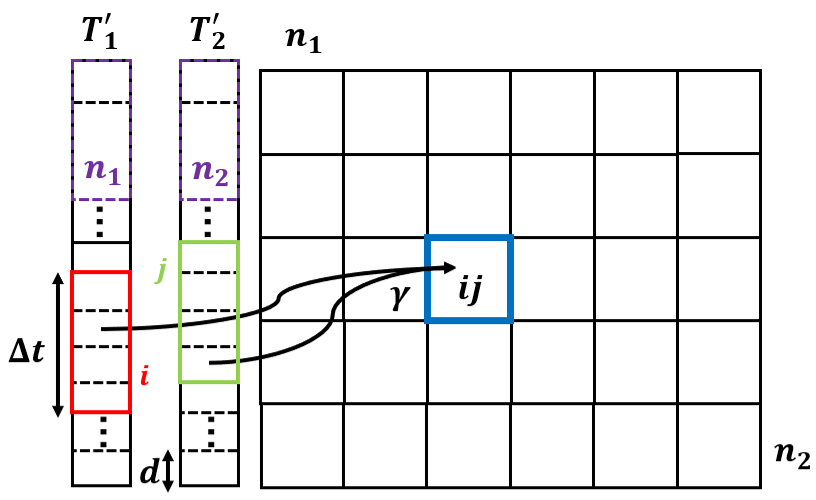
\includegraphics[scale=0.61]{Imagenes/idea.png}
    \caption{Esquema del desplazamiento de una ventana de tiempo sobre las series temporales y el cálculo de la función cross-correlation entre pares de ventanas de tiempo.}
    \label{scan}
\end{figure}

En la figura \ref{scan} se muestra gráficamente la idea detrás cálculo de las funciones de correlación, para una ventana de amplitud $\Delta t$. El tiempo de desplazamiento ($d$) de cada ventana sobre las series temporales, en las $n_{1}$ y $n_{2}$ particiones, permite encontrar los intervalos de tiempo que están más correlacionados. La exactitud de estos intervalos está determinada por el tamaño del desplazamiento. En este trabajo se toma un valor lo suficientemente pequeño en comparación con la duración de las series temporales.

El barrido sobre el lapso de las ventanas de tiempo consiste en calcular la función cross-correlation, como se muestra en la figura \ref{scan}, desde una ventana de amplitud mínima a una de amplitud máxima. Esto genera tantas matrices de correlaciones como amplitudes de ventanas. 

Cabe señalar que los barridos propuestos se realizaron en Python, debido a la facilidad de implementación, manejo y almacenamiento de variables. En el anexo \ref{xcorr_scan_code} se adjunta el código en Python para realizar estas cuentas. Los resultados se almacenan en la variable ${\tt params\char`_time}$ al hacer iterar la función  ${\tt params\char`_xcorr}$ en el ciclo que barre las diferentes ventanas de tiempo.  

Ahora, veamos un ejemplo del cálculo de la función cross-correlation entre un par de ventanas. Tomando $d = 7$ minutos y $\Delta t = 27$ minutos entonces el número de celdas que se obtienen para PSP y SolO son $n_{1} = 15$ y $n_{2} = 31$, respectivamente. En la figura \ref {scan:example1} se muestra la función cross-correlation entre la ventana 10 de la sonda PSP y la ventana 20 de la sonda SolO. El intervalo de tiempo correspondiente en PSP es $04:25 - 04:52$ UT del 27 de septiembre de 2020 y el intervalo de tiempo en SolO es $23:05 - 23:32$ UT del 01 de octubre de 2020. El máximo de correlación es 0.37 y se obtuvo con un desfase de 9.67 minutos entre las series temporales.

\begin{figure}[H]
    \centering
    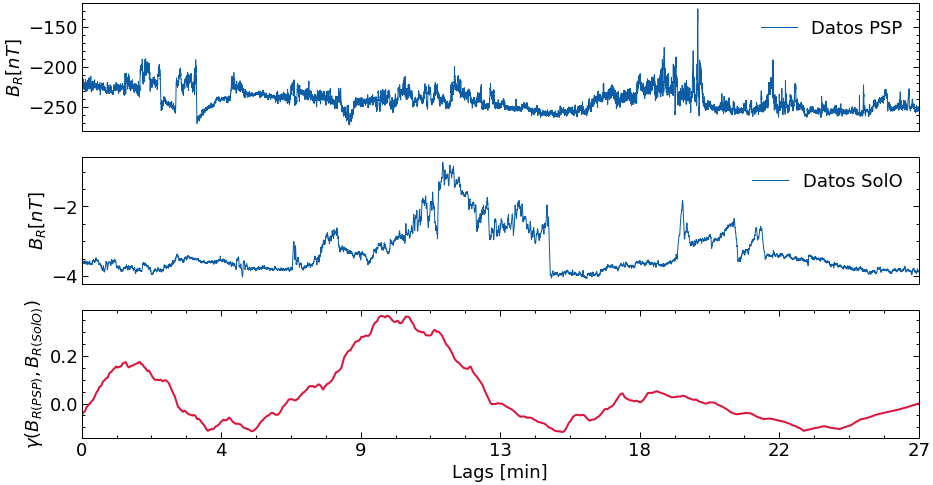
\includegraphics[scale=0.445]{Imagenes/scan_example1.png}
    \caption{Cross-correlation entre los datos de PSP y SolO en una ventana de 27 minutos. De arriba hacia abajo: ventana en PSP, ventana en SolO, función cross-correlation.}
    \label{scan:example1}
\end{figure}

Recordemos que el desfase es el tiempo que se desplazan los datos de una serie temporal respecto de la otra en el cálculo de la función cross-correlation. Aquí reportamos el desfase donde la función de correlación es máxima. Esta magnitud podría contener información física de relevancia, y se debería estudiar sobre aquellos pares de ventanas que presentan la máxima correlación. En nuestro estudio no se ha hecho esto, pero es algo que se podría investigar en un análisis exploratorio futuro. 

Hasta ahora hemos explicado la idea de cómo evaluamos la correlación entre ventanas de dos series. Sin embargo, uno de nuestros objetivos principales es hacer estos cálculos entre las series resultantes de un proceso de filtrado, donde las componentes de alta frecuencia hayan sido eliminadas. Así, primero nos interesa descomponer las series en sus IMFs. Luego se hacen reconstrucciones parciales, al ir disminuyendo las IMFs, hasta quedarnos con un número determinado de aquellas componentes correspondientes a las bajas frecuencias. Y tras cada reconstrucción, calculamos las correlaciones. El número de IMFs que necesitemos considerar, para obtener resultados significativos en el cálculo de las correlaciones, es una de las cosas que queremos determinar en este trabajo.

Este procedimiento se realiza para cada amplitud de ventana. También, como las series pueden descomponer en un número diferente de componentes, en este barrido, la serie con el menor número de IMFs limita las componentes filtradas de la otra serie. Cuando ambas series tienen el mismo número de IMFs entonces el filtro termina con la componente de menor frecuencia más el residuo.       

En la figura \ref {scan:example2} se muestran las reconstrucciones de las ventanas de tiempo de la figura \ref {scan:example1} y su función cross-correlation. Cada reconstrucción se realiza con 5 IMFs. Al reducir las altas frecuencias, los valores de la función de correlación aumentan respecto de la curva de la figura \ref {scan:example1}. El máximo de correlación es 0.42 con un desfase de 9.70 minutos.

\begin{figure}[H]
    \centering
    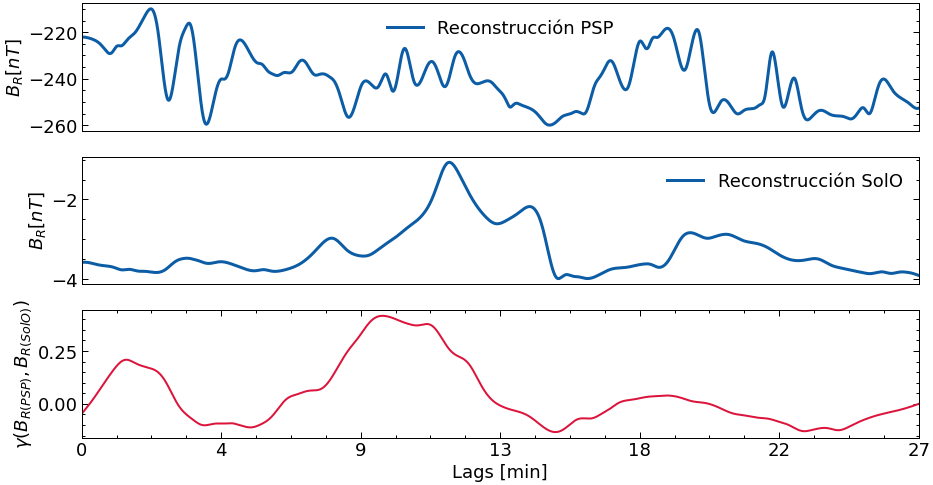
\includegraphics[scale=0.445]{Imagenes/scan_example2.png}
    \caption{Similar a \ref{scan:example1} aunque con los datos (de las ventanas) reconstruidos con las primeras 5 IMFs de baja frecuencia.}
    \label{scan:example2}
\end{figure}

Los cálculos se ejecutaron con las IMFs obtenidas de la implementación del método EMD en Fortran y aquellas resultantes de una implementación en Python \cite{quinn_emd_2021}. Esto se hizo para comparar los resultados obtenidos en Fortran con los de una implementación profesional del EMD. En esta última se fijó el valor límite del criterio de detenimiento del proceso \textit{sifting} en $SD^{*} = 0.3$, como en la implementación de Fortran. 

En nuestro código de Python del anexo \ref{xcorr_scan_code} estas cuentas se muestran para la implementación del EMD de Python. La función ${\tt params\char`_xcorr}$ ejecuta el barrido sobre las IMFs para cada valor de ventana. El residuo y las IMFs extraídas de las series se almacenan en las columnas de un arreglo bidimensional. Las columnas de este arreglo se pueden sumar fácilmente en Python, especificando las columnas a sumar. El arreglo (columna) resultante es la reconstrucción parcial de una serie.

Para cada valor de ventana, todas las posibles correlaciones entre pares de particiones de las series se realizan en un doble ciclo. En cada iteración se calcula el máximo de correlación. Estos valores se ordenan de mayor a menor a través de la función ${\tt get\char`_jixcorrs}$ y se registran en la variable ${\tt max\char`_vals}$. Junto a estos valores se almacenan los índices de las particiones de cada serie. También, para cada máximo de correlación, se evalúa y se almacena el desfase entre cada par de ventanas. De esta manera, el primer valor contiene el máximo de todas las posibles correlaciones y las particiones asociadas. 

Una ligera modificación de la función ${\tt params\char`_xcorr}$ permite efectuar el barrido con los resultados de Fortran. En este caso, las IMFs se introducen externamente como variables globales. Primero, como ya no se utiliza la implementación del EMD en Python, se retiran los parámetros asociados. Luego, se elimina el parámetro de entrada ${\tt field\char`_component}$ así como la lectura de las componentes que se realiza con este parámetro. Finalmente, en esta parte se cargan las IMFs y se limita la duración de las series temporales con los valores de $T'$ correspondientes.

Por último, cabe señalar que las funciones mencionadas son de autoria propia y son las que permiten extraer información del barrido. Dentro de estas funciones se utilizan otras funciones propias de Python para realizar procedimientos de soporte, por ejemplo, la función que permite realizar la descomposición de las series temporales mediante el método EMD. 